\documentclass[12pt]{article}

% Set page size and margins
\usepackage[a4paper,top=2.54cm,bottom=2.54cm,left=2.54cm,right=2.54cm,marginparwidth=1.75cm]{geometry}
\usepackage{setspace} 
\onehalfspacing

\usepackage{indentfirst}
\setlength{\parindent}{1cm}

% Authors and affiliation package
\usepackage{authblk}

% Referencing
\usepackage[numbers,sort&compress]{natbib}
\bibliographystyle{apalike}

% Hyperlinks
\usepackage[colorlinks=true, allcolors=blue]{hyperref}

% Lists
\usepackage{enumitem}

% AMS math 
\usepackage{amsmath}

% Graphics support
\usepackage{graphicx}
\usepackage{float}
\usepackage{subcaption}
\usepackage{tikz}
\usetikzlibrary{positioning,arrows.meta}

% Color support
\usepackage{xcolor}

% Tables
\usepackage{booktabs} 
\usepackage{caption} 
\usepackage{array}  % 用于表格对齐

% Unnumbered footnotes
\newcommand\blfootnote[1]{%
  \begingroup
  \renewcommand\thefootnote{}\footnote{#1}%
  \addtocounter{footnote}{-1}%
  \endgroup
}

% 标题美化设置
\usepackage{titling}
\usepackage{mathpazo}  % Palatino 字体
% 自定义标题格式
\renewcommand{\maketitle}{
\begin{center}
    \vspace*{-0.3cm}


% 主标题 - Palatino 粗体
{\fontsize{24pt}{28pt}\selectfont\bfseries\rmfamily
Automated Email Response System for Customer Service\par}

\vspace{0.3cm}

% 副标题 - Palatino 小型大写
{\large\scshape MIS2001 Intermediate Report\par}
    
    \vspace{0.5cm}
    
    % 作者信息 - 三列对齐
    {\normalsize
    \begin{tabular}{*{3}{c}}
    Liu Liwei 122040083 & Li Yunjia 122020098 & Gao Jiabao 122090121 \\[0.8ex]
    Xiang Xiyuan 122090598 & Wu Shenyu 123090626 & Li Zongguo 123030038
\end{tabular}\par}
    
    \vspace{0.3cm}
    
    % 装饰线和日期
    \centerline{{\color{gray!40}\rule{1.0\textwidth}{0.8pt}}}
    \vspace{0.4cm}
\end{center}
\thispagestyle{empty}
}

\begin{document}
\maketitle

\section{Introduction}
With the rapid development of e-commerce and global trade, the need for communication between businesses and customers has increased significantly. In the logistics and international trade industries, email remains one of the primary channels for customer service communication. Customers typically use email to inquire about order status, shipping progress, billing issues, and after-sales service. 

However, as business operations expand, customer service teams must handle a large volume of repetitive emails daily. This not only increases labor costs but also leads to longer response times, which in turn affects customer satisfaction. Traditional manual email processing methods are no longer sufficient to meet businesses’ demands for high efficiency and high-quality service. Against this backdrop, automated customer service systems have gradually become a key focus of corporate digital transformation. 

This project aims to design and implement an AI-based automated email response system. By leveraging natural language processing and large language model technologies to automatically analyze and respond to customer emails, the system will enhance customer service efficiency, reduce operational costs, and improve the overall customer experience.




\section{Industry Context \& Market Opportunity }
In the logistics and international trade industries, communication between customers and businesses is extremely frequent due to cross-border transportation, multi-party collaboration, and complex supply chain management. Customers typically use email to inquire about order status, shipping progress, customs clearance information, as well as billing and invoicing issues. At the same time, because of differences in time zones, a large volume of customer emails are sent outside of business hours, placing additional pressure on customer service teams to respond. It is worth noting that a significant portion of these emails contains highly repetitive content—such as price inquiries and estimated arrival times—which presents an ideal use case for automated processing.

Against this backdrop, the application of artificial intelligence (AI) technology in the customer service sector is rapidly expanding and demonstrating significant market potential. According to reports from market research firms, the global AI customer service market is projected to grow from approximately \$12.06 billion in 2024 to \$47.8 billion by 2030, with a compound annual growth rate (CAGR) of over 25\%. This growth is primarily driven by rising demand from businesses for automated customer service systems, natural language processing (NLP) technology, and intelligent response tools. The adoption of AI customer service systems can help reduce operational costs and significantly improve service efficiency, thereby enabling businesses to enhance response times while optimizing the customer experience.

From a regional perspective, the Asia-Pacific region is one of the fastest-growing markets for AI customer service. In China, in particular, the application of intelligent customer service systems has reached a relatively mature stage, with enterprise adoption rates continuing to rise. Driven by the trend of digital transformation, an increasing number of companies are adopting automated tools to address high-frequency, repetitive customer communication needs.

In summary, the issue of repetitive emails in the logistics industry, combined with the rapid growth of the AI market, indicates that AI-based automated email response systems possess significant practical value and a promising future.

\section{Problem Statement \& Existing Solutions}

The logistics industry faces persistent operational inefficiencies in customer service email management, driven by high email volumes, repetitive task workflows, and slow response times. These problems directly translate into significant business negative impacts: On one hand, manual processing is time-consuming and labor-intensive, increasing the enterprise's operating costs; on the other hand, delayed responses and inconsistent services continuously reduce customer satisfaction, weakening the core competitiveness of the enterprise in the fierce market competition.

Current approaches to managing logistics customer service emails suffer from critical limitations that fail to fully address industry-specific needs. The current solutions mainly include basic email filtering rules, static reply template libraries, CRM integration automatic reply tools, and general AI writing assistance tools. However, these tools all have five core problems:

• Insufficient Intent Recognition Accuracy: Basic filters and templates cannot precisely distinguish complex intentions in logistics scenarios or interpret the nuanced intent of logistics inquiries, leading to misclassification and irrelevant responses.

• No Human-in-the-Loop Oversight: Many autoresponders lack a confidence scoring mechanism and human-machine collaboration mechanism, meaning high-risk or complex emails are automated without human review, increasing the chance of errors and customer dissatisfaction.

• Data Security \& Compliance Risks: Cloud-based AI tools often store email content on external servers, violating data privacy regulations and exposing sensitive shipment and customer data.

\section{Project Objectives}

This project aims to develop an automatic email response assistant for the logistics industry. While automating the processing of routine customer service emails, it retains the processing authority of human operators for complex scenarios that require empathy and judgment.

Specific goals include:

• Automate repetitive tasks to free up customer service staff for high-value work;

• Shorten the response time of emails to improve customer service efficiency.

• Reduce enterprise operating costs and optimize manpower allocation.

• Maintain human supervision to ensure the quality of services in complex scenarios and risk controllability.

\section{Our Solution: Automatic Email Responder}

We propose a domain-specific Automatic Email Responder designed for the logistics industry. Through four core functions, intent recognition, dynamic response generation, confidence-based routing, and local data storage, it addresses the pain points of existing solutions.

• Intent Recognition \& Auto-categorization: Uses NLP to classify incoming emails into predefined logistics categories. Automatically archives and tags emails for efficient retrieval and reporting.

• Context-aware Auto-reply Generation: it retrieves order and goods data in real time, dynamically generates reply content that fits the scenario, and supports style adaptation and tone adjustment to ensure the accuracy and consistency of the replies.

• Confidence-based Human-in-the-Loop Routing: For each automatic reply, a confidence score is assigned. High-confidence emails are directly sent automatically, while low-confidence emails are transferred to human agents for review before being sent, achieving a balance between efficiency and security.

• Local Data Storage \& Compliance: Stores all emails and generated replies locally or on a private cloud, ensuring full compliance with data privacy regulations and avoiding the risk of sensitive business information leakage. Meanwhile, all processing records are retained to facilitate traceability and auditability.

\section{System Architecture}\label{sec:system-architecture}

\subsection{Overview}
The system follows a conventional three-tier pattern: a browser-based single-page application (SPA), a local Flask REST API, and integrations with external cloud services. The frontend talks to the backend over HTTP; the backend reads and sends Outlook mail via Microsoft Graph API, performs classification and reply generation through an OpenAI-compatible API, and persists state and audit data in a local SQLite database. A company product catalog is maintained as a JSON file and exposed through a dedicated service and API for reply templates.

\begin{figure}[htbp]
\centering
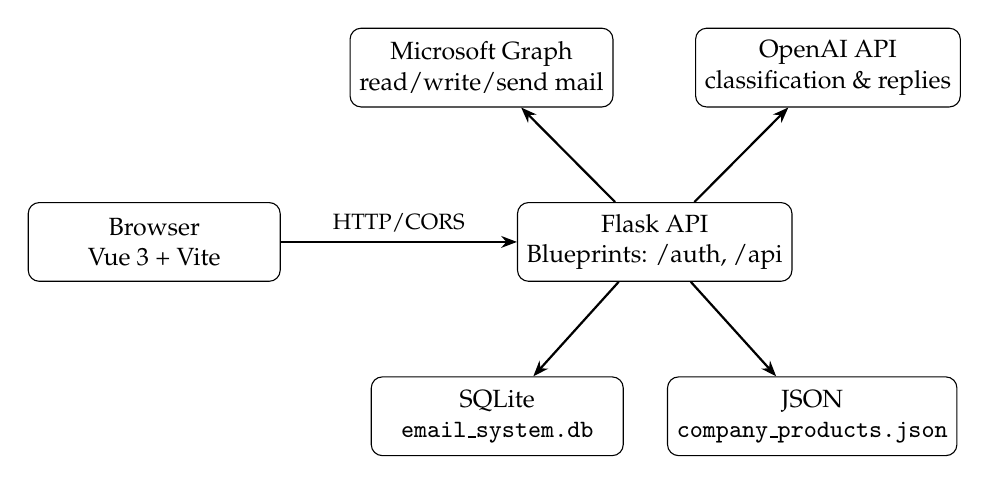
\begin{tikzpicture}[
  font=\small,
  box/.style={draw, rounded corners, minimum width=3.2cm, minimum height=1cm, align=center},
  arrow/.style={-{Stealth[length=2mm]}, thick}
]
\node[box] (fe) {Browser\\Vue 3 + Vite};
\node[box, right=3cm of fe] (api) {Flask API\\Blueprints: /auth, /api};
\node[box, below=1.2cm of api, xshift=-2cm] (db) {SQLite\\\texttt{email\_system.db}};
\node[box, below=1.2cm of api, xshift=2cm] (json) {JSON\\\texttt{company\_products.json}};
\node[box, above=1.2cm of api, xshift=-2.2cm] (graph) {Microsoft Graph\\read/write/send mail};
\node[box, above=1.2cm of api, xshift=2.2cm] (llm) {OpenAI API\\classification \& replies};

\draw[arrow] (fe) -- node[midway, above=2pt, font=\footnotesize, inner sep=1pt] {HTTP/CORS} (api);
\draw[arrow] (api) -- (db);
\draw[arrow] (api) -- (json);
\draw[arrow] (api) -- (graph);
\draw[arrow] (api) -- (llm);
\end{tikzpicture}
\caption{Logical layers and main external dependencies}
\label{fig:arch}
\end{figure}

\subsection{Server-side responsibilities}
\begin{itemize}
  \item \textbf{Authentication:} OAuth2 via Azure AD (Microsoft Identity Platform); the server maintains a session holding tokens and profile attributes required to invoke Microsoft Graph on behalf of the authenticated user.
  \item \textbf{Mail operations:} Endpoints support ingesting new messages, listing and filtering threads with pagination, retrieving a single message together with its draft reply, and sending or approving outbound replies. Mailbox access and message submission are mediated by Graph; responsibilities are partitioned into dedicated modules for Graph integration, classification, and reply generation.
  \item \textbf{Product catalog:} The backend validates and maintains a product inventory used in reply composition (e.g.\ prices and lead times), exposed through REST-style operations alongside the mail workflow.
  \item \textbf{Persistence:} Messages, generated replies, classification scores, workflow status (pending review, auto-sent, ignored without reply, send failed), deduplication keys, and basic audit metadata are stored locally so that the interface can restore prior state and present historical outcomes without depending solely on the language model.
\end{itemize}

\subsection{Intelligent processing pipeline}
\begin{enumerate}
  \item \textbf{Rule pre-filter:} Prior to any large-model invocation, lightweight keyword checks on the subject and body flag correspondence that is clearly non-operational or noisy, reducing the likelihood of misclassification.
  \item \textbf{Two-stage classification:} An initial relevance stage determines whether the message constitutes a logistics- or trade-related service inquiry. When affirmative, a second stage assigns one of seven operational categories and returns a confidence score together with a concise rationale in structured form.
  \item \textbf{Reply and send policy:} Each category maps to either a template-based response or free-form generation. A global confidence threshold governs whether a draft may be dispatched automatically or must await human approval; for non-business items, a short fixed explanation may still be recorded for audit purposes even when no outbound message is sent.
  \item \textbf{Robustness:} Messages are processed independently so that a single failure does not halt the remainder of a batch. Outbound delivery employs retries with exponential backoff; persistent failures are recorded explicitly to enable operator intervention and to avoid silent loss of error information.
\end{enumerate}

\subsection{Client application}
The user interface is implemented as a Vue~3 single-page application comprising views for authentication, inbox-style listing, message detail, and an aggregate dashboard. In development, a Vite development server hosts the UI and proxies API requests to the backend; an optional launcher script may start the API and static assets concurrently to support a streamlined local evaluation setup.


\section{Preliminary Results}

This section summarizes staged outcomes from the project development record and observed runtime behavior, in terms of \textbf{functionality} and \textbf{observability}. It does not report large-scale offline benchmark metrics.

\subsection{Classification and business safety}
\begin{itemize}
  \item \textbf{Seven labels} are implemented (pricing, cancellation, tracking, shipping time, shipping exception, billing/invoice, non-business) and aligned with the reply template system.
  \item \textbf{Two-stage decisions} reduce the chance that system notifications or marketing mail are treated as business correspondence and trigger automatic replies; non-business items converge on dedicated workflow states (e.g.\ ignored without outbound reply), with optional fixed templates for traceability.
  \item \textbf{Rules + model} provide a practical fallback for noisy traffic and are easier to control in production than a single-shot LLM classifier alone.
\end{itemize}

\subsection{End-to-end flow and operations visibility}
\begin{itemize}
  \item \textbf{Batch fetch resilience:} Bulk ingestion processes each message independently so that one failure does not abort the remainder; responses summarize how many items were processed, skipped, or failed, and give an aggregate breakdown by outcome.
  \item \textbf{Latency and rates:} The service reports total and per-message processing time where applicable; dashboard-style views can expose the share of non-business traffic, send failure rates, and related ratios as specified during development.
  \item \textbf{Send reliability:} Retries and explicit failure marking make delivery problems visible and actionable rather than failing silently.
\end{itemize}

\subsection{Content and data support}
\begin{itemize}
  \item \textbf{Templates:} Core categories have template or fixed-format paths (e.g.\ billing-style replies), reducing stylistic drift.
  \item \textbf{Company catalog:} A structured on-disk product directory, updated through backend catalog operations, grounds pricing-related replies in maintained data.
\end{itemize}

Together, these results show a \textbf{closed loop} (fetch---classify---draft---send/review) and \textbf{risk controls} (thresholds, non-business handling, traceable failures) suitable for demo and iteration. For publication-grade ``preliminary results,'' a next step would be quantitative evaluation on a fixed test set (accuracy, latency percentiles, human edit rate).

\section{Prototype Demonstration}

This section illustrates the working prototype through representative interface screenshots. The flow begins with secure access to the application, continues with inbox-style triage and operational visibility, and ends with the three principal outcomes of the pipeline: confident automatic replies, deliberate non-reply for non-business traffic, and human-reviewed sending when automation is withheld.


\begin{figure}[H]
  \centering
  \includegraphics[width=0.4\textwidth]{figures/Login.png}
  \caption{Login Interface}
  \label{fig:login}
\end{figure}

Figure~\ref{fig:login} shows the entry point. Authentication is required before any mailbox data or generated drafts are exposed, which mirrors production expectations for access control and auditability.


\begin{figure}[H]
  \centering
  \includegraphics[width=0.8\textwidth]{figures/Interface.png}
  \caption{Main Interface}
  \label{fig:main}
\end{figure}

Figure~\ref{fig:main} presents the primary operator view. Users can scan incoming messages, inspect inferred categories and confidence, and drive the next step (e.g.\ refresh, batch processing, or opening a thread for detail), supporting the closed loop described in Section~\ref{sec:system-architecture}.


\begin{figure}[H]
  \centering
  \includegraphics[width=0.8\textwidth]{figures/Statistic.png}
  \caption{Response Statistics}
  \label{fig:stats}
\end{figure}

Figure~\ref{fig:stats} complements the per-message list with roll-up statistics. Such visibility helps validate batch behavior, spot send failures, and compare business versus non-business volume without exporting raw logs.

\begin{figure}[H]
  \centering
  \includegraphics[width=0.8\textwidth]{figures/Auto-response.png}
  \caption{Auto Response}
  \label{fig:autores}
\end{figure}

Figure~\ref{fig:autores} demonstrates the intended benefit of automation for repetitive, well-scoped inquiries. The interface should make it obvious that a reply was generated and sent under the configured policy, preserving traceability for later audits.

\begin{figure}[H]
  \centering
  \includegraphics[width=0.8\textwidth]{figures/Auto-ignorance.png}
  \caption{Auto Ignorance}
  \label{fig:autoign}
\end{figure}

Figure~\ref{fig:autoign} highlights the safety-oriented branch for traffic that should not trigger customer-facing automation. Ignoring with a clear system state reduces noise in the outbox while still documenting why no reply was sent.

\begin{figure}[H]
  \centering
  \includegraphics[width=0.8\textwidth]{figures/Manual-response.png}
  \caption{Manual Response}
  \label{fig:manualres}
\end{figure}

Figure~\ref{fig:manualres} shows the review path for uncertain or high-stakes cases. Manual approval closes the gap between throughput and reliability, matching the project objective of combining model assistance with operator judgment.

\section{Challenges}

Several practical constraints shaped design and implementation.

\textbf{Heterogeneous real mail.} Logistics and trade emails rarely follow a single pattern: one message may mix tracking, quotation, and billing; content may be short and vague or long yet incomplete. Simple keyword rules or a single classifier are insufficient. The system must separate business from irrelevant traffic and assign a stable category.

\textbf{Automation versus reliability.} Speed matters, but incorrect auto-replies erode trust and create rework. The pipeline must estimate confidence, flag uncertain cases, and route high-risk items to human review---automation should cut repetition, not remove judgment where stakes are high.

\textbf{LLM-as-judge and confidence.} Using a large language model as a judge does not produce confidence estimates that are reliably calibrated or externally verifiable; the model's response alone is insufficient to decide automatic sending versus human escalation. The workflow therefore cannot treat LLM-reported certainty as ground truth and must combine explicit thresholds, safeguards, and review paths rather than delegating that boundary to the model in isolation.

\textbf{Stable classification and reply quality.} Even when mail is business-related, nearby categories (e.g.\ tracking, shipping time, exceptions) can be confused. Replies must stay professional and policy-aligned. A two-stage classifier, non-business fallbacks, and template paths improved consistency; quality still depends on prompts, thresholds, and post-processing.

\textbf{Operational robustness.} Beyond text classification, the system must tolerate send failures, API instability, and partial batch errors so one bad message does not stop the rest---hence retries, explicit failure states, and traceable errors.

\textbf{Privacy and auditability.} Processing customer mail and outbound drafts involves sensitive data. Microsoft login, Outlook authorization, and stored review records improve realism; a production deployment would need stronger access control and compliance.

\section{Work Distribution}

\textbf{Jiabao Gao (122090121).} Contributed to implementation and ongoing maintenance of the automated email response system, including debugging and iterative improvements; helped draft parts of the report, notably the system architecture material and adjacent technical sections.

\section{Project Timeline}

Development moved from scope to a working prototype in stages.

\textbf{Planning and requirements.} The team framed communication pain points in logistics and trade (repetitive mail on quotes, status, shipping, billing), defined scope, and set the objective: faster responses with human oversight where needed.

\textbf{System design.} Main modules were fixed (intent classification, automated replies, review, dashboard) and the stack chosen: web UI, Flask API, Graph for mail, OpenAI for classification and generation, SQLite for local state.

\textbf{Workflow refinement.} A one-shot classifier proved too brittle; the flow gained rule filtering, a business-relevance gate, category assignment, and confidence-based routing to reduce misclassification and unsafe auto-sends.

\textbf{Prototype build.} Features were implemented incrementally: Microsoft sign-in, Outlook fetch, category classification, draft generation, non-business paths, review, and dashboard. Later additions included retries, error logging, and a structured product catalog.

\textbf{Current phase.} Focus shifts to tighter testing, model tuning, and end-to-end polish---an iterative path rather than a single release.

\section{Future Work}

Priority improvements before treating the system as production-ready include the following. Taken together, they respond to the challenges above: heterogeneous mail and stable categories, safe automation, limits of LLM-as-judge confidence, reply quality, operational robustness, and privacy---while allowing additional scope beyond that list.

\textbf{Classification and heterogeneous mail.} Richer prompts, few-shot examples, and explicit logic for borderline, incomplete, and multi-intent messages would better match real logistics and trade traffic (e.g.\ a single thread mixing tracking, quotation, and billing; very short or overly long bodies that obscure intent).

\textbf{Rubric-guided LLM scoring.} To address unreliable free-form confidence from LLM-as-judge, we plan fixed \emph{rubrics} that require the model to score each case against explicit criteria instead of a single opaque verdict. Two rubrics are envisaged: one for \emph{classification} confidence (e.g.\ clarity of intent, support for the chosen category versus plausible alternatives), and one for \emph{auto-send readiness} of the generated reply (e.g.\ factual grounding against retrieved or stated facts, completeness relative to the request, tone and policy fit). Rubric outputs would still be combined with thresholds and human review, and periodically checked against operator labels so scores are treated as guidance, not ground truth.

\textbf{Confidence routing and review policy.} Building on rubric scores and existing flags, category-specific or adaptive thresholds and rules informed by past reviews could replace a single global cutoff where data supports it, preserving the automation--reliability balance.

\textbf{Reply generation and policy-aligned quality.} Expanding the product knowledge base and scenario templates would improve drafts when adjacent categories are easily confused, keeping tone, urgency, and policy alignment consistent with the classification stage.

\textbf{Operational resilience.} Beyond current retries and explicit failure states, future work includes clearer monitoring and alerting, predictable degradation when APIs fail, and stronger batch isolation and recovery so one bad message or transient outage does not obscure the rest of the queue.

\textbf{Privacy, access control, and audit.} A production deployment would add role-based access, data minimization and retention policies for mail and drafts, and auditable records of classification, rubric scores, and auto-send vs.\ manual decisions for compliance and post-incident review.

\textbf{Testing and evaluation.} Broader unit and integration tests plus user-facing or rubric-assisted evaluation would surface edge cases, estimate mis-route and unsafe auto-send rates, and validate the full workflow end-to-end.

\textbf{Scope.} Possible extensions include multilingual support, deeper CRM or order-system integration, and additional service scenarios.

\section{Conclusion}

This project responds to a concrete need: logistics and trade teams spend heavy time on repetitive customer email, yet delays and inconsistency still hurt experience. We proposed an automated customer service email workflow combining intent classification, AI-generated drafts, confidence-based routing, manual review, and dashboard management.

The contribution is not only ``use AI for email'' but a workable pipeline: Outlook access via Microsoft Graph, predefined categories, two-stage classification, non-business filtering, draft generation, and traceable outcomes---aligned with real operational constraints.

Intelligent service here does not mean full replacement of staff. The design targets repetitive, lower-risk work while leaving uncertain or sensitive cases to humans---a balance that matters when communication errors have operational impact.

Overall, combining NLP, large language models, and careful workflow design shows clear promise for this domain. The prototype still limits accuracy, flexibility, and evaluation depth, but it offers a credible base for further work and demonstrates both technical and business relevance as a course project.

\end{document}

\end{document}
